\documentclass[]{article}

\usepackage{graphicx}
\graphicspath{ {./../graphics/} }
%opening
\title{trees wip}
\author{Max Caragozian}

\begin{document}
	


\maketitle

\section{Preface}
The  American West has the largest, tallest, and oldest trees in the world. Those superlative trees, however, are often found in environments that are harsh either due to their aridity or their bitter winters. While the high mountains of the Sierra Nevada and the Transverse Ranges have consistent yearly precipitation in the form of winter snow, plants lower down depend on fickle rains that sometimes fail for years on end.

In the home of the world's oldest trees, tree rings encode that climate in a history stretching back almost two thousand years. Interpreting that history and using it to make predictions about the future is of huge practical value, as California has the largest agricultural output of any state. Sierra Nevada snowmelt trapped in resevoirs and Colorado River water pumped in by aqueduct irragate most of those farms. Tree rings give climate scientists a window into how the snowpack and rivers looked hundreds of years in the past, which is only becoming more important in the era of climate change.

I grew up in Los Angeles and spent weekends and summers tromping around the natural wonderland that California has to offer. I gained an appreciation for the sheer variety of climates and ecosystems the West contains. Chaparall with regal old oaks, subalpine forests with fir and pine, alpine tundra where krumholzed lodgepole pines cling to the edge of the tree line: All can be found within thirty miles of Los Angeles, and each biome brings back warm memories for me. I learned very quickly that in Southern California, a good year for plants is synonymous with a wet year. I aim to use tree ring and historical data to quantify that relationshoip and investigate how climate change might affect it. 

\section{Sources and Locations}
The tree ring data I use come from the study \textit{University of Arizona Southern California Tree-Ring Study} by D. M. Meko, C. A. Woodhouse, and E. R. Bigio \cite{tree_study}. The authors used tree ring data to construct estimates of historical river flow. In addition to publishing their hydrological reconstructions, the authors also published the tree ring width datasets on which those reconstructions were built. One important consideration is that the tree ring width data not raw. The authors ``detrended'' the data to remove long-term biological noise such as the effects of a tree aging, and the result is that the each ring width datapoint is a unitless quantity and not an actual measure of length. See secion 2.1 of the study for more details\cite{tree_study}.

The study covers 29 collection sites distributed among three broad regions: Southern California, the Southern Sierra Nevada, and the Upper Colorado River basin. The collection sites in Southern California are 3000-9000ft above sea level, lying somewhere along the transition from chaparall to alpine forest, while the Southern Sierra sites are around 10,000ft and recieve significant winter snows despite being on the eastern (rain shadow) side of Sierra Crest. The Upper Colorado Basin Sites are in typical Great Basin environemnts: 6000-9000ft. above sea level and arid. 

\begin{figure}
	\centering
	\includegraphics[width=0.8\textwidth]{baldy.png}
	\caption{Typical Southern California Transverse Range scene. Mount Baldy (10,064') background center-right}
	\label{fig:baldy}
\end{figure}

\begin{figure}
	\centering
	\includegraphics[width=0.8\textwidth]{cottonwood_lakes.png}
	\caption{High Sierra Meadow in summer after heavy snow year. Mount Langley (14,032') center-right.}
	\label{fig:cottonwood}
\end{figure}

\begin{figure}
	\centering
	\includegraphics[width=0.8\textwidth]{arch.jpg}
	\caption{Skyline Arch at Arches National Park \cite{arch_pic}.}
	\label{fig:arch}
\end{figure}

Weather data proved trickier to find. Many of the sites where tree samples were taken are in remote areas that don't have extensive weather records. To get around this, I took my climate data from an arbitrary city in each region: Los Angeles, CA for Southern California, Bishop, CA, for the Southern Sierra, and Moab, UT for the Upper Colorado River Basin. \textbf{The climate these cities might differ significantly from the climate at the sample sites.  The city weather data are just a proxy for the whole region's climate in a given year.} For example, consider the Eastern Sierra, where I used weather data from Bishop, CA. Bishop is in the rain shadow of the Sierra Nevada and recieves significantly less precipitation than  the mountains that surround it. During the period 1993-2016, Bishop averaged 4.71 inches of precipitation per year,  while Mammoth Lakes, only 35 miles away, averaged 22.95.However, although Mammoth Lakes and Bishop may have very different climates, a relatively wet in year in one town will also be realtively wet and the other. 

\begin{figure}
	\centering
	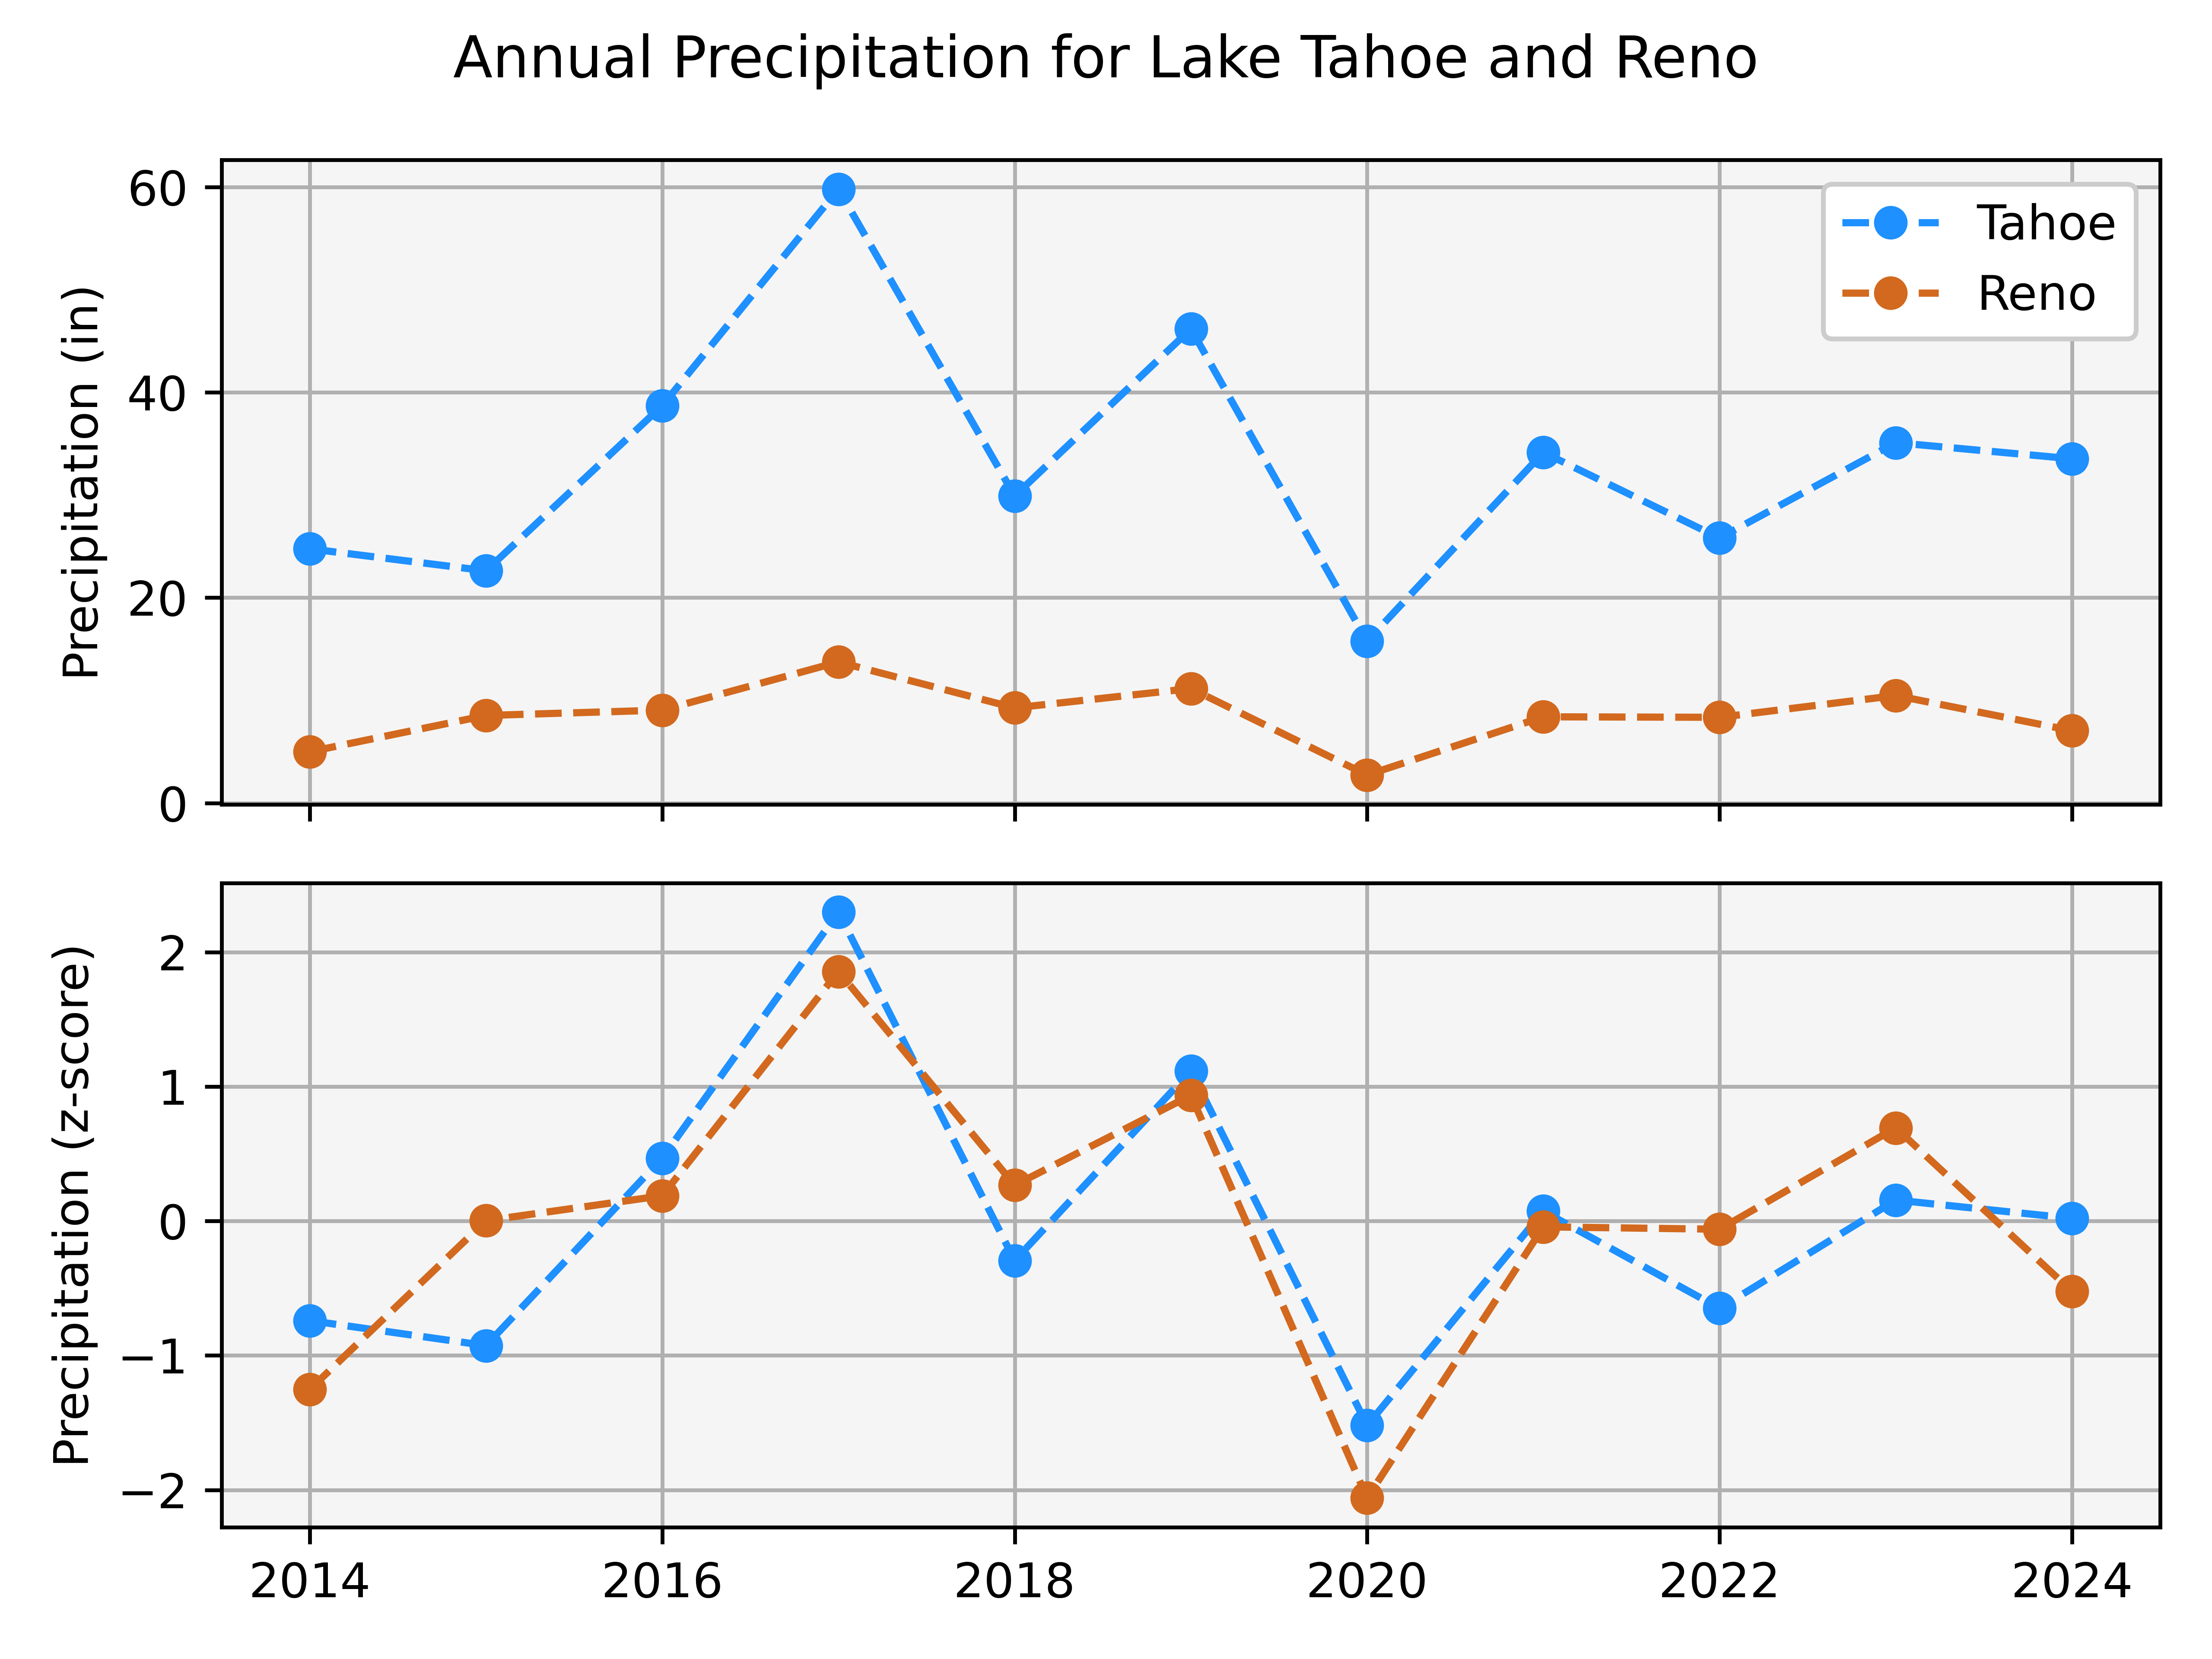
\includegraphics[width=0.8\textwidth]{renotahoe.png}
	\caption{Annual precipitation for Tahoe City and Reno over a 10 year period. The top plot shows absolute rain values in inches, and the bottom plot shows each datapoint as a z-score.}
	\label{fig:reno_tahoe}
\end{figure}
We can clearly see that trend in figure \ref{fig:reno_tahoe}, which plots rainfall for another pair of cities: Tahoe City in the Sierra Nevada and Reno in its rain shadow. Although Tahoe City gets around four times as much precipitation as Reno, if we normalize the data for each city seperately we can see that they almost always trend the same way; a year that sees one standard deviation above average rainfall in Reno will likely see precipitation one standard deviation above the average in Tahoe City.

The upshot is that we can confidently describe historical weather trends at tree ring collection sites even if the nearest weather station is tens of miles away and in a drastically different climate. Unless noted otherwise, all statistical calculations use the scaled and normalized weather data. I have only preserved the absolute values where comparisons between regions requires it.

\section{What Weather Makes the Trees Happy?}
The first question I aim to answer is how tree ring growth relates to short term variation in climate. Is my childhood notion that trees like a wet year supported by the data?  I made scatter plots plotting observed tree ring growth against the scaled rainfall and temperature.

\begin{figure}
	\centering
	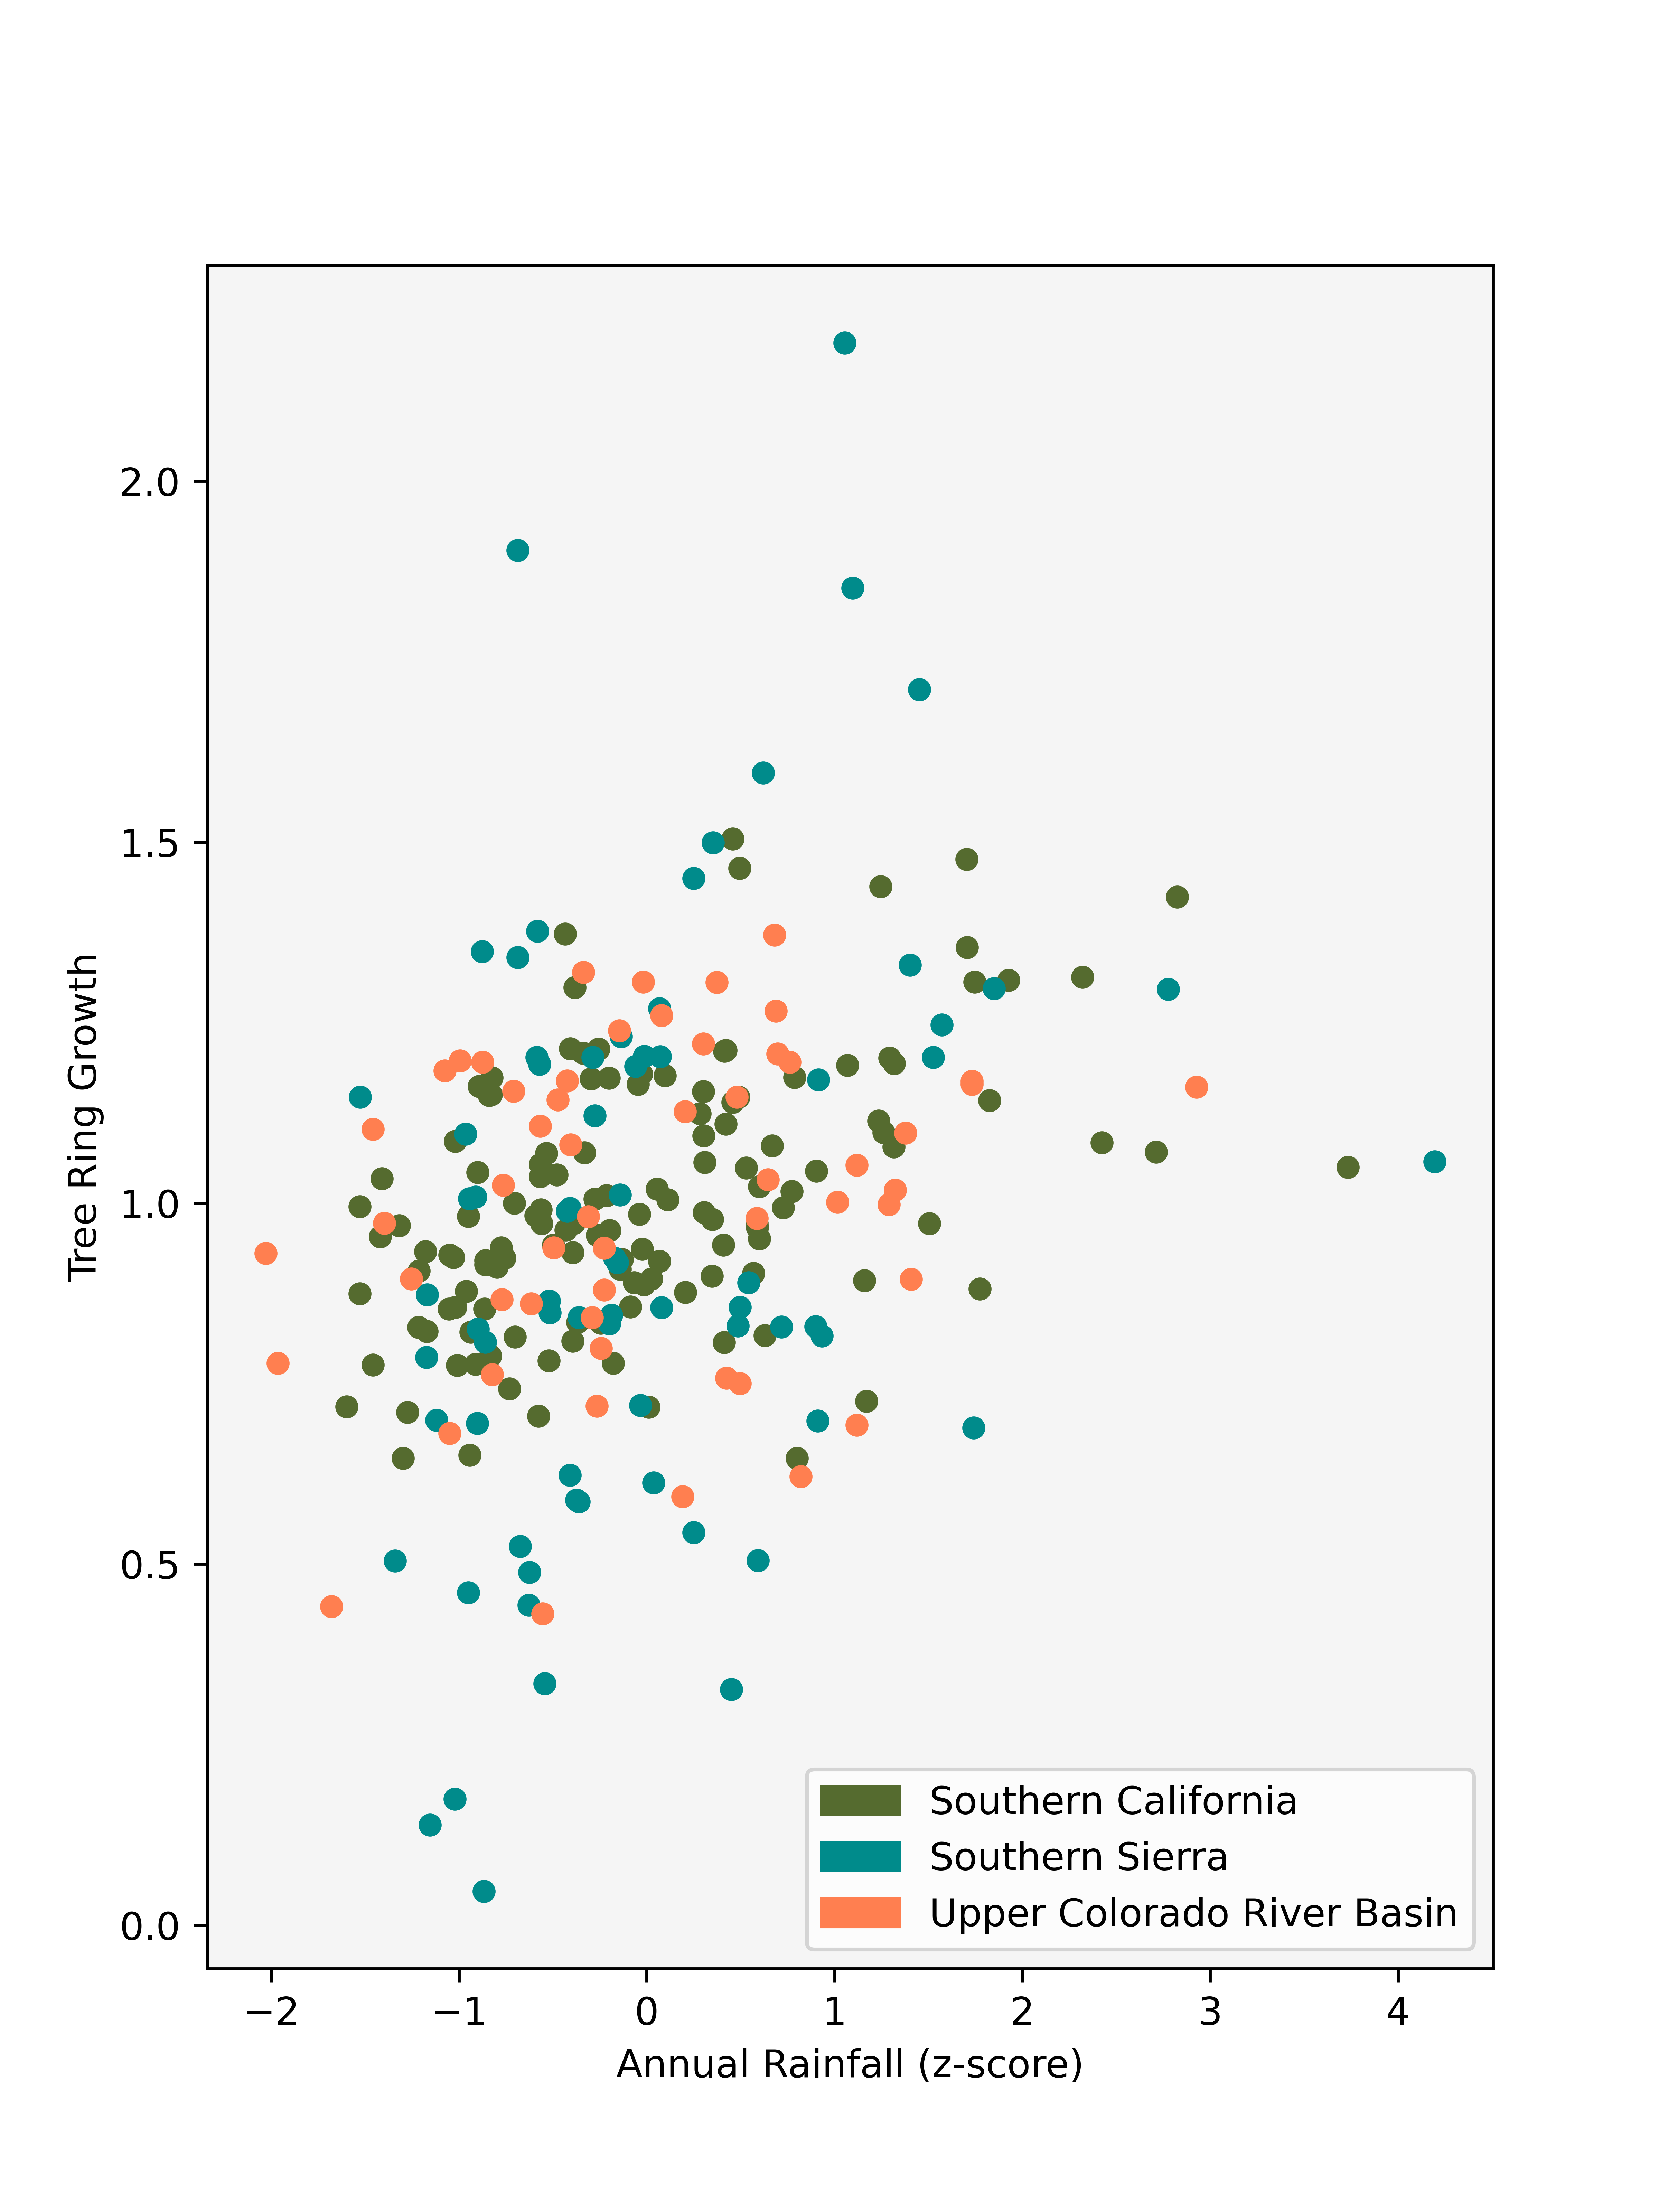
\includegraphics[width=0.4\textwidth]{precip_scatter.png}
	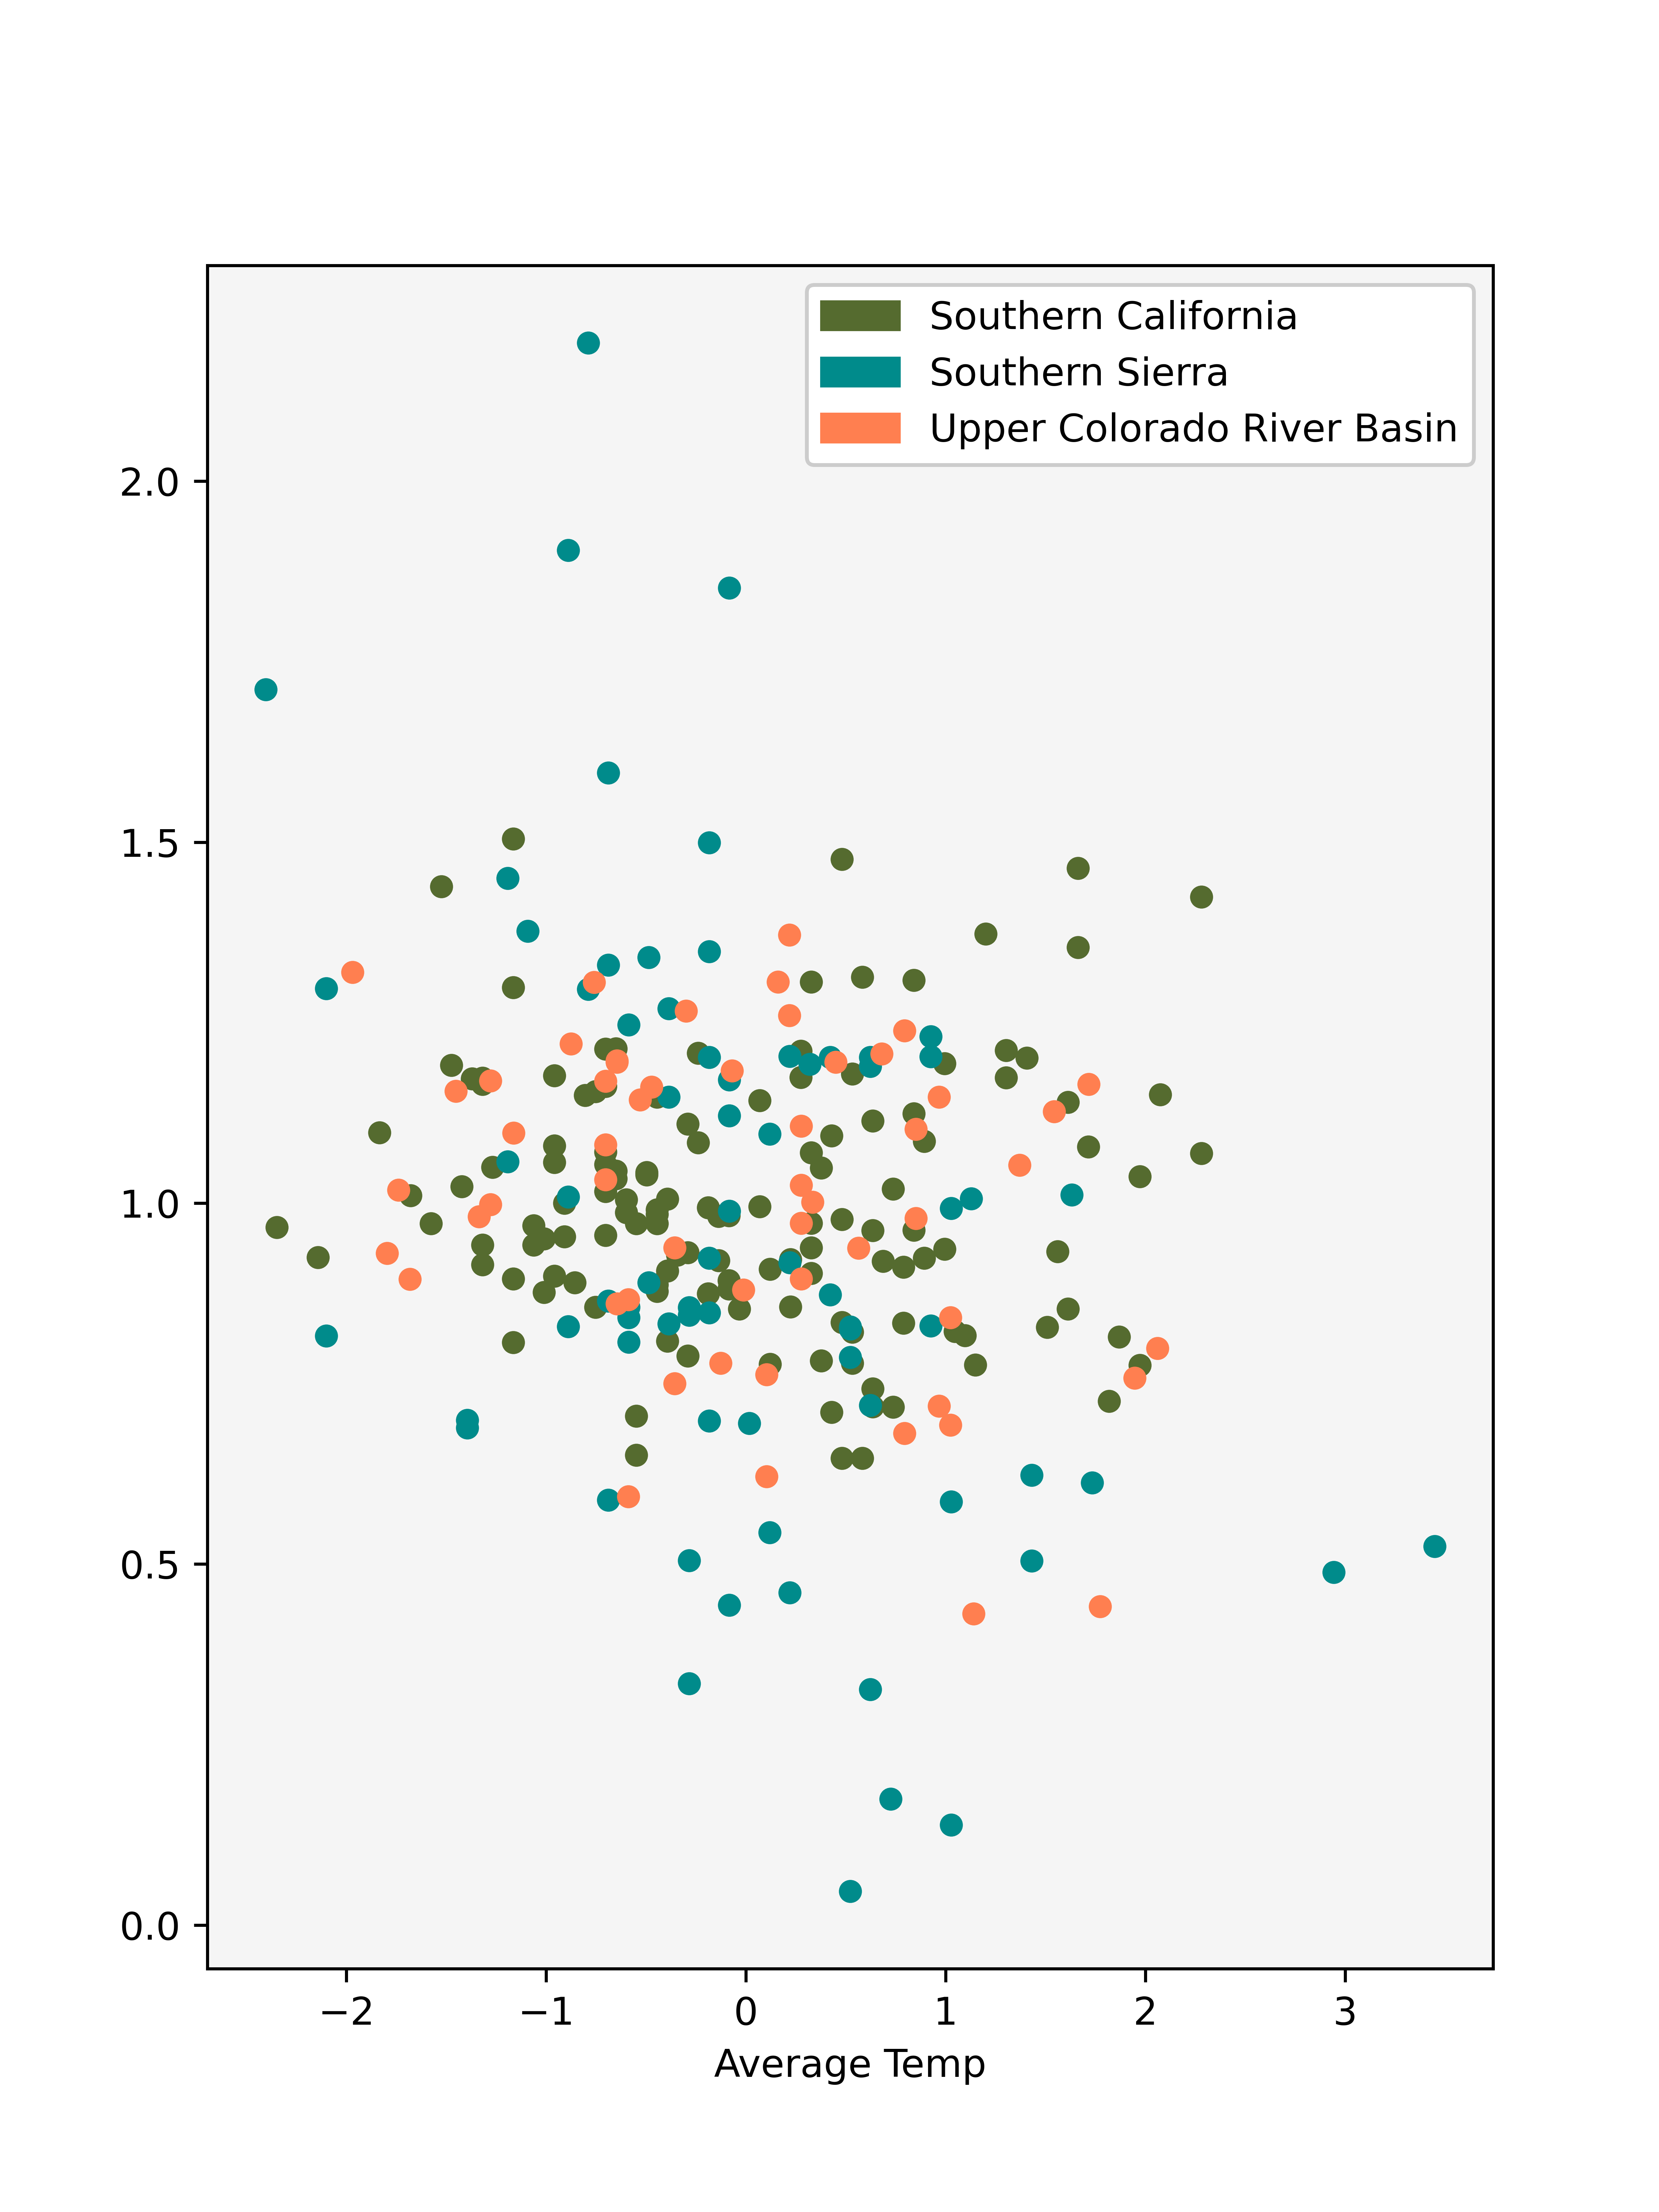
\includegraphics[width=0.4\textwidth]{temp_scatter.png}
	\caption{Scatter plots of tree ring width versus precipitation and temperature. The dots are colored according to which region the datapoint comes from.}
\end{figure} 






\begin{thebibliography}{9}
	\bibitem{tree_study}
	D. M. Meko, C. A. Woodhouse, and E. R. Bigio, “University of Arizona
	Southern California Tree-Ring Study,” California Department of Water Resources, Feb. 2017, Accessed: Feb. 27, 2025. [Online].
	
	\bibitem{weather_data}
	“AgAcis.” https://agacis.rcc-acis.org
	
	\bibitem{arch_pic}
	S. Acharya, The Skyline Arch at Arches National Park, Utah, USA. 2009.
\end{thebibliography}


\end{document}
